% Compile check only: Experimental Setup + Methodology + Results in IEEEtran conference format.
\documentclass[conference]{IEEEtran}
\usepackage{amsmath,amssymb}
\usepackage{graphicx}
\usepackage{array}
\usepackage{ragged2e}

\begin{document}
\title{CHAI-FP: Characterizing Hierarchical AI Model Fingerprints from Network Traffic Metadata}
\author{\IEEEauthorblockN{Compile check}}
\maketitle
\begin{abstract}
Federated learning (FL) keeps training data on client devices, but the network
traffic it generates can still reveal which model is being trained. We present
CHAI-FP, a framework that characterizes how much AI model identity a passive
observer can infer from packet-level metadata alone, without inspecting payloads
or model parameters. CHAI-FP reconstructs the round structure of FL traffic and
identifies models hierarchically at the family, architecture, and variant
levels. Its key element is cross-device fingerprinting. Because FL clients train the
same model on heterogeneous hardware and operating systems, the differences
between their traffic reveal the architecture's compute profile. On a physical testbed with three
heterogeneous clients (two Ubuntu, one Windows) and 32 experiments spanning convolutional, recurrent,
transformer, and autoencoder models, cross-device fingerprinting identifies the
family of unseen models with a balanced accuracy of 0.74, compared with 0.58 for
per-client classification, and raises family accuracy in 5~s windows from 0.31
to 0.51. Within a family, the architecture is identified with a mean balanced
accuracy of 0.79 from complete traces, and convolutional architectures with 0.71
from 5~s windows. The model payload size is a baseline leak that reveals the
exact variant in every trace, and in 69\% from a single model download within
a 5~s window, but it is removed by padding, whereas family identification from
timing alone remains at 0.62, showing that concealing model
identity in FL requires timing defenses in addition to size padding.
\end{abstract}

\begin{IEEEkeywords}
Federated learning, traffic analysis, side channels, model fingerprinting,
network security, privacy.
\end{IEEEkeywords}

\section{Introduction}
\label{sec:introduction}
Artificial intelligence (AI) workloads are increasingly executed across edge
devices, cloud services, and distributed learning
systems~\cite{zhou2019edge,mcmahan2017communication}. Although encryption and
access controls protect transmitted content and model artifacts, they do not
conceal all characteristics of the communication generated during execution:
packet sizes, directions, timing, volumes, and burst patterns remain observable
to a network intermediary~\cite{sirinam2018deep}. Such metadata may reveal
properties of an AI workload even when the observer cannot inspect model
parameters, application data, or payloads~\cite{shuvo2025fingerprinting}.
Federated learning (FL) is particularly exposed, because every training round
produces a characteristic exchange in which each client downloads the global
model, trains locally, and uploads an update.

\textbf{Existing Research:} Prior studies infer neural network information from
indirect execution observations, including memory accesses, shared caches, GPU
execution traces, and system resource
measurements~\cite{hua2018reverse,yan2020cache,hu2020deepsniffer,patwari2022dnn}.
These observations require physical access to, or co-location with, the
executing device. Network traffic is a more remote observation surface, on which
communication protocols, training schedules, transport behavior, and network
conditions may obscure architectural differences. Encrypted-traffic analysis
reveals visited
websites~\cite{panchenko2011website,wang2014effective,hayes2016kfingerprinting,sirinam2018deep},
and PACKETPRINT~\cite{li2022packet} identifies mobile applications and user
activities from encrypted wireless packet sequences, although its hierarchy
captures traffic patterns rather than structural relationships among AI models.
For AI workloads, network traffic has been used to discriminate CNN and RNN
families in FL~\cite{shuvo2025fingerprinting}, to classify CNN and RNN
architectures and variants from encrypted wireless traffic with results reported
primarily at the family level~\cite{shuvo2026flare}, to identify AI applications
and their execution phases~\cite{oyaniyi2026fingerprinting}, and to identify AI
families from 5G scheduling metadata~\cite{shuvo2026flint}.

\textbf{Gap:} The extent to which passive network observations reveal the
structural identity of AI models beyond the family level remains insufficiently
characterized. It is not established whether an observer can progressively
distinguish families, architectures, and variants, how much of this information
is available within short observation windows, or whether it survives
countermeasures such as size padding. Moreover, existing approaches classify each
client's traffic independently and do not exploit a defining property of FL:
all clients train the same model concurrently on heterogeneous hardware and
operating systems.

\textbf{Motivation:} Three technical challenges motivate this investigation.
First, different families and architectures may generate similar communication
patterns under common FL protocols, so network similarity is an imperfect
indicator of model structure. Second, discriminative characteristics of complete
traces may be unavailable within short windows, which capture only portions of a
round. Third, observations from the same execution are correlated, so randomly
distributing them between training and testing produces optimistic estimates;
generalization must instead be assessed on models absent from training.
Architectural leakage also has security consequences. Knowledge of a model's
family, architecture, or variant narrows the range of potential targets and
helps an adversary select relevant attack techniques, for instance by training a
surrogate of the matching architecture for model extraction or transfer-based
adversarial attacks~\cite{TODO-model-extraction}, and it exposes proprietary
design choices.

\textbf{This Work:} We present CHAI-FP, a conditional hierarchical framework
that infers the family, architecture, and variant of the model under training
from passive packet metadata. CHAI-FP reconstructs the round structure of FL
traffic, from which it derives communication features and a passive estimate of
local training time, the compute gap between model download and upload, and it
combines the traffic of all clients into a cross-device representation. We
evaluate it on a physical FL testbed with three clients that differ in both
hardware and operating system, and 32
experiments, using model-disjoint validation on 0.5 to 5~s windows and complete
traces.

\noindent\textbf{Contributions:} The contributions of this study are threefold.
(i)~A conditional hierarchical fingerprinting framework that identifies model
families, architectures, and variants from passive network metadata, combining
packet-morphology features with compute-timing features derived from the FL
round structure; within a family, packet-morphology features identify the
architecture with a mean balanced accuracy of 0.79.
(ii)~Cross-device fingerprinting, which exploits the heterogeneous clients of a
federated job to raise family identification of unseen models from 0.58 to 0.74
for complete traces and from 0.31 to 0.51 for 5~s windows, where it also
identifies convolutional architectures with 0.71; an ablation shows that the gain requires both
the cross-device representation and a regularized linear classifier.
(iii)~A model-disjoint evaluation of the observable leakage, showing that
payload size is a baseline leak that reveals the exact variant in every trace,
and in $69\%$ from a single model download within a 5~s window, but is
removed by padding, whereas family identification from timing
alone remains at 0.62, so that concealing model identity requires timing
defenses.

The remainder of the paper is organized as follows.
Section~\ref{sec:setup} describes the experimental setup,
Section~\ref{sec:methodology} presents the CHAI-FP framework,
Section~\ref{sec:results} reports the results,
Section~\ref{sec:discussion} discusses countermeasures, and
Section~\ref{sec:conclusion} concludes the paper.


% Placeholder for the system architecture figure (replace with your PDF).
\begin{figure}[!t]
\centering
\fbox{\parbox[c][3cm][c]{0.9\columnwidth}{\centering Placeholder: system architecture figure}}
\caption{Overview of the hierarchical AI fingerprinting framework.}
\label{fig:architecture}
\end{figure}

\section{Experimental Setup}
\label{sec:setup}
The experimental testbed consists of three AI execution clients, a coordinating
server, and a passive network proxy positioned along the communication path.
The testbed is heterogeneous in both hardware and operating system: the clients
are an NVIDIA Jetson Orin Nano and a Dell desktop running Ubuntu, and a Dell
laptop running Windows~11, whereas the server, hosted on an NVIDIA Jetson AGX
Orin, and the proxy run Ubuntu. The clients therefore differ in compute
capability as well as in their network stacks; for example, the Windows client
omits the TCP timestamp option that the Ubuntu hosts use by default. In two
experiments, the Jetson AGX Orin also served as the embedded client. Clients
connect to the proxy, which relays their traffic to the server, so every
client--server exchange traverses the observation point. The proxy captures packet-level metadata, including packet
sizes, directions, timing, traffic volumes, and burst characteristics, without
accessing model parameters or application payloads. These quantities are
observable whether or not the payload is encrypted. Table~\ref{tab:ai_workloads}
summarizes the AI workloads, architectural configurations, and training
datasets. Each experiment executes 100 federated learning rounds. Federated
training uses a custom synchronous FedAvg implementation in PyTorch, in which
the server and clients exchange length-prefixed messages over TCP; in each
round, every client downloads the global model, trains locally, and uploads one
update before the server aggregates and advances to the next round. The
experimental corpus comprises 32 independent experiments and 96 client-level
aggregated observations. Traffic is represented using 0.5, 1, 2, and 5~s
observation windows and complete-trace aggregates to examine fingerprinting
performance across temporal scales. Classification is evaluated across the
family, architecture, and variant levels of the model hierarchy, with the
validation protocol detailed in Sec.~\ref{subsec:classification}.

\begin{table}[!htbp]
\centering
\caption{AI Workloads, Architectures, Variants, and Datasets}
\label{tab:ai_workloads}
\scriptsize
\renewcommand{\arraystretch}{1.10}
\setlength{\tabcolsep}{2pt}
\begin{tabular}{
>{\RaggedRight\arraybackslash}p{0.19\columnwidth}
>{\RaggedRight\arraybackslash}p{0.22\columnwidth}
>{\RaggedRight\arraybackslash}p{0.32\columnwidth}
>{\RaggedRight\arraybackslash}p{0.16\columnwidth}
}
\hline
\textbf{Family} &
\textbf{Architecture} &
\textbf{Representative Variants} &
\textbf{Dataset} \\
\hline
Autoencoder &
Dense, Conv., VAE &
Layer configurations, $\beta$-VAE, Conv. VAE &
Fashion-MNIST \\
CNN &
ResNet, MobileNet, EfficientNet &
ResNet18/34/50/101, MobileNetV2/V3,
EfficientNet-B0/B1/B2 &
Fashion-MNIST \\
RNN &
LSTM, GRU &
Single-layer, multilayer,
bidirectional variants &
UCI HAR \\
Transformer &
BERT, DistilBERT, Tiny Transformer &
BERT model sizes,
lightweight configurations &
AG News \\
\hline
\end{tabular}
\end{table}

\section{Methodology}
\label{sec:methodology}
The proposed hierarchical AI fingerprinting framework identifies AI model
characteristics from network side-channel observations without requiring access
to application payloads or model parameters. As illustrated in
Fig.~\ref{fig:architecture}, the framework consists of passive traffic
observation, multiscale feature extraction, hierarchical classification, and
fingerprint evaluation.

\subsection{Fingerprinting Dataset and Ground Truth}
\label{subsec:dataset}
The dataset comprises about 499 million packets (670~GB, 190~hours of traffic)
from 32 experiments, one per variant, each observed from three clients
(Table~\ref{tab:fp_dataset}). Each of the 96 client traces yields one
complete-trace observation and a sequence of windows; round-level quantities
are available for the 90 traces whose rounds are fully reconstructed. Because
larger models produce longer traces, training weights every experiment equally.
Each observation is described by 68 size-normalized features covering direction
and volume ratios, transmission rates, and packet-size, interarrival, burst, and
idle statistics. Complete traces add nine compute-timing features derived from
the round structure, giving 77 features per client and 231 in the cross-device
representation~\eqref{eq:crossdevice}. Labels and per-model metadata (parameter
count, serialized size, and training FLOPs per sample) are computed from the
model source code and are used only for evaluation.

\begin{table}[!htbp]
\centering
\caption{Fingerprinting Dataset Composition}
\label{tab:fp_dataset}
\scriptsize
\renewcommand{\arraystretch}{1.05}
\setlength{\tabcolsep}{4pt}
\begin{tabular}{lccccc}
\hline
\textbf{Family} & \textbf{Arch.} & \textbf{Var.} & \textbf{Traces} &
\textbf{5~s win.} & \textbf{0.5~s win.} \\
\hline
Autoencoder & 3  & 9  & 27 & 7{,}943  & 57{,}786 \\
CNN         & 3  & 9  & 27 & 35{,}947 & 298{,}965 \\
RNN         & 2  & 6  & 18 & 2{,}578  & 12{,}036 \\
Transformer & 3  & 8  & 24 & 39{,}585 & 345{,}817 \\
\hline
\textbf{Total} & \textbf{11} & \textbf{32} & \textbf{96} & \textbf{86{,}053} & \textbf{714{,}604} \\
\hline
\end{tabular}
\end{table}

\subsection{Data Preprocessing}
\label{subsec:preprocessing}
Raw captures are converted into analysis-ready traces in five steps.

\emph{Trace assembly.} For every client connection, the proxy records a sequence
of packet entries (timestamp, frame length, direction, and TCP flags). Long
experiments are captured in consecutive chunks, which are placed on a common
timeline using their recorded capture-start offsets, and each trace is mapped to
its client device through the client address logged by the proxy. Connection
attempts that complete no training round are discarded.

\emph{Payload recovery.} The TCP payload of each packet is obtained by
subtracting the Ethernet, IPv4, and TCP header length from the frame length.
The header length is inferred per connection from the size of pure
acknowledgments: 66 bytes when the TCP timestamp option is used and 54 bytes
when it is not, as on the Windows client.
Packets without payload, such as pure acknowledgments, are excluded from
transfer reconstruction.

\emph{Transfer and round reconstruction.} Transfers are recovered as maximal
runs of same-direction data packets, tolerating small opposite-direction control
packets (at most 300~B) and transient stalls caused by wireless retransmission,
which must not split a transfer. Because rounds alternate strictly between
download and upload, the model-carrying transfers are identified as the
byte-weighted dominant size class in each direction, and each upload is paired
with the preceding download to delimit a round.

\emph{Windowing and filtering.} Each trace is segmented into non-overlapping
windows on the global timeline (Sec.~\ref{subsec:multiscale}). Windows with
fewer than 20 packets are discarded, and near-idle windows are additionally
removed for cross-device window classification.

\emph{Normalization.} Features that scale directly with model size or trace
length (absolute byte and packet counts, durations, and connection and TCP flag
counts) are excluded, so that the remaining features describe the shape of the
traffic rather than its volume. Missing and non-finite values, which arise for
windows without traffic in one direction or for an absent device in the
cross-device representation, are set to zero for windows and to the feature
median for traces. Features are standardized using statistics computed on the
training folds only.

\subsection{Traffic Observation and Feature Extraction}
Network traffic exchanged between AI clients and the coordinating server is
observed at an intermediate proxy. Each captured packet is represented by
observable metadata, including its timestamp, size, and communication direction.
Let
\begin{equation}
p_i = (t_i, s_i, d_i)
\label{eq:packet}
\end{equation}
denote the $i$th observed packet, where $t_i$ is its arrival timestamp, $s_i$ is
its size, and $d_i$ indicates its communication direction. From the resulting
packet sequence, the framework extracts statistical features describing packet
sizes, interarrival times, directional traffic volumes, transmission rates, and
burst behavior.

Beyond per-packet statistics, we exploit the round structure of federated
training. Each round consists of a model download, a local-training interval
with no traffic, and a model upload. From the directional packet sequence we
recover, for round $k$, the end of the download $t^{\mathrm{d}}_{k}$ and the
start of the upload $t^{\mathrm{u}}_{k}$, and define the \emph{compute gap}
\begin{equation}
g_k = t^{\mathrm{u}}_{k} - t^{\mathrm{d}}_{k},
\label{eq:gap}
\end{equation}
a passive proxy for local training time that excludes the inter-client
synchronization wait. Together, these measurements form a network fingerprint
representing the communication and computation characteristics of the executing
AI workload. The per-trace summary augments the packet-morphology features with
the compute gap normalized by uploaded payload, its dispersion, and cross-device
timing ratios (Sec.~\ref{subsec:crossdevice}).

\subsection{Multiscale Traffic Representation}
\label{subsec:multiscale}
To investigate the temporal availability of AI fingerprints, the observed
traffic is represented at multiple time scales. For an observation duration
$\Delta$, packets are grouped into temporal windows, and a feature vector is
computed for each window:
\begin{equation}
\mathbf{x}_{k}^{(\Delta)}
=
\phi\left(
\{p_i \mid k\Delta \leq t_i < (k+1)\Delta\}
\right),
\label{eq:window_features}
\end{equation}
where $\phi(\cdot)$ denotes the traffic feature extraction function. The
framework considers observation durations $\Delta \in \{0.5,1,2,5\}$~s. In
addition, complete client traces are summarized into aggregated fingerprints to
characterize communication behavior over the entire observed execution.

A single short window observes only a fragment of one round. We therefore
aggregate a client's window-level posteriors to a trace-level decision by
averaging,
\begin{equation}
P(y \mid \mathcal{T})
= \frac{1}{|\mathcal{T}|}\sum_{k \in \mathcal{T}}
P\!\left(y \mid \mathbf{x}_k^{(\Delta)}\right),
\label{eq:pooling}
\end{equation}
where $\mathcal{T}$ indexes the windows of a trace. This recovers the
round-level signal lost to short windows without additional training, and
enables comparison between short-duration traffic signatures and complete-trace
observations.

For cross-device window classification, the three clients' windows covering
the same global interval are concatenated, analogously to~\eqref{eq:crossdevice}.
Near-idle windows, whose transferred bytes fall below $5\%$ of the trace's
busy-window volume or whose retransmission share exceeds $5\%$, are removed
before classification; this filter is fixed in advance and uses no labels.
For short windows, variant identity is assessed by nearest-reference matching on
the size of a model download that completes within the window.
To study observation times beyond the window length, the posteriors of
consecutive 5~s windows are averaged with~\eqref{eq:pooling} over
non-overlapping spans of 10 to 30~s.

\subsection{Hierarchical AI Model Fingerprinting}
Rather than treating all AI models as unrelated classes, the proposed framework
represents model identity through a three-level hierarchy:
\begin{equation}
\mathcal{H} =
\mathcal{F}
\rightarrow
\mathcal{A}
\rightarrow
\mathcal{V},
\label{eq:hierarchy}
\end{equation}
where $\mathcal{F}$, $\mathcal{A}$, and $\mathcal{V}$ denote model families,
architectures, and variants, respectively. Given a network fingerprint
$\mathbf{x}$, family identification is performed as
\begin{equation}
\hat{f}
=
\arg\max_{f \in \mathcal{F}}
P(f \mid \mathbf{x}).
\label{eq:family}
\end{equation}
Architecture identification is then conditioned on the selected family:
\begin{equation}
\hat{a}
=
\arg\max_{a \in \mathcal{A}(\hat{f})}
P(a \mid \mathbf{x},\hat{f}),
\label{eq:architecture}
\end{equation}
where $\mathcal{A}(\hat{f})$ denotes the architectures associated with the
selected family. Finally, variant identification is conditioned on the selected
architecture:
\begin{equation}
\hat{v}
=
\arg\max_{v \in \mathcal{V}(\hat{a})}
P(v \mid \mathbf{x},\hat{a}),
\label{eq:variant}
\end{equation}
where $\mathcal{V}(\hat{a})$ represents the candidate variants belonging to the
selected architecture. This hierarchical formulation preserves the structural
relationships among AI models and enables fingerprinting at progressively finer
levels of model identity. To isolate per-level discriminability, each level is
also evaluated independently using the ground-truth parent.

\subsection{Cross-Device Fingerprinting}
\label{subsec:crossdevice}
In federated learning, the participating clients train the \emph{same} model on
heterogeneous hardware and operating systems. Classifying each client in isolation discards the most
discriminative cue available to a passive observer: how the timing and transfer
shape of the identical model differ \emph{across} devices, which is governed by
the architecture's per-layer compute profile. We therefore represent each
experiment $e$ by a single feature vector that concatenates the per-device
summaries,
\begin{equation}
\mathbf{x}_e =
\big[\,
\mathbf{f}^{(1)}_{e} \,\Vert\,
\mathbf{f}^{(2)}_{e} \,\Vert\,
\mathbf{f}^{(3)}_{e} \,\Vert\,
\mathbf{r}_e
\,\big],
\label{eq:crossdevice}
\end{equation}
where $\mathbf{f}^{(c)}_{e}$ is the size-normalized feature vector of client $c$
and $\mathbf{r}_e$ collects cross-device compute-gap and throughput ratios.
Because~\eqref{eq:crossdevice} yields few high-dimensional examples, family
identification~\eqref{eq:family} is performed with an $\ell_2$-regularized
multinomial logistic regression whose regularization strength is chosen by
nested cross-validation (Sec.~\ref{subsec:classification}); tree ensembles
overfit this regime.

\subsection{Feature Selection, Classification, and Validation}
\label{subsec:classification}
The extracted traffic fingerprints train supervised classifiers for each
hierarchical identification task. Feature discriminability is examined using
Fisher-score-based selection, which evaluates the separation between classes
relative to their within-class variability, and is performed independently
within each training fold to prevent information leakage from held-out
executions. For the per-client representations we use Fisher-selected random
forests; for the cross-device representation~\eqref{eq:crossdevice} we use
regularized logistic regression. Exact-model identification is performed by
nearest-reference matching on the logarithm of the uploaded payload size.

Generalization is assessed under experiment-disjoint, leave-one-model-out
validation, in which every held-out model is absent from training, so
performance measures recognition of unseen models rather than memorization. All
hyperparameter and feature-selection choices are made within an inner loop over
the training models, so held-out executions never influence model selection.
Performance is reported as balanced accuracy, whose chance level is
$1/|\mathcal{C}|$ for a $|\mathcal{C}|$-class task, independent of class sizes;
reliability is quantified by a group-bootstrap $95\%$ confidence interval over
models and a label-permutation test against chance.

At the variant level, each model is realized by a single execution, and variant
identity is recovered through exact-model identification: every variant produces
a distinct serialized size, enabling nearest-reference matching on the uploaded
payload. Confusion matrices and feature discriminability are examined to
characterize residual ambiguity among AI workloads, particularly where different
architectures exhibit similar network communication patterns.

Robustness to size concealment is assessed by simulating a padding defense in
which every transfer is padded up to a size bucket, and by repeating family
identification using only features independent of transfer size: the compute
gap, its dispersion, and cross-device gap ratios.

\section{Results}
\label{sec:results}
We report fingerprinting performance at the family, architecture, and variant
levels, then for short observation windows and under a size-padding defense.
Scores are balanced accuracy, for which chance is $1/|\mathcal{C}|$.

\subsection{Family Identification}
Table~\ref{tab:family_methods} compares family identification methods. Under the
repeated protocol used for the earlier methods (20 seeds $\times$ 5-fold
model-disjoint cross-validation), the cross-device representation
of~\eqref{eq:crossdevice} achieves $0.68 \pm 0.04$, the highest among all
methods evaluated this way (fixed late fusion: 0.61) and 0.20 above a per-client
random forest ($0.48 \pm 0.04$). Under leave-one-model-out validation, which
trains on all remaining models, it reaches 0.74 (95\% CI 0.58--0.88, macro F1
0.74), significantly above chance (permutation test, $p = 0.003$), compared with
0.58 for the per-client random forest. Recurrent networks are identified without
error (6/6), convolutional networks in 7 of 9 cases, autoencoders in 6 of 9, and
transformers in 4 of 8 (Fig.~\ref{fig:family_confusion}). The remaining errors
involve architectures whose compute per parameter overlaps.

\begin{table}[!htbp]
\centering
\caption{Family Identification (4 classes, chance 0.25)}
\label{tab:family_methods}
\scriptsize
\renewcommand{\arraystretch}{1.08}
\setlength{\tabcolsep}{3pt}
\begin{tabular}{lcc}
\hline
 & \multicolumn{2}{c}{\textbf{Balanced accuracy}} \\
\textbf{Method} & \textbf{Repeated CV} & \textbf{Leave-one-model-out} \\
\hline
306-feature morphology (RF)        & 0.55 & -- \\
Compute-per-byte                   & 0.57 & -- \\
Fixed late fusion                  & 0.61 & -- \\
Equal-probability hybrid fusion    & 0.68$^{*}$ & -- \\
Per-client RF                      & 0.48 & 0.58 \\
\textbf{Cross-device LR (proposed)} & \textbf{0.68} & \textbf{0.74} \\
\hline
\end{tabular}

\vspace{2pt}
\parbox{0.95\columnwidth}{\scriptsize Repeated CV: mean over 20 seeds
$\times$ 5-fold model-disjoint cross-validation. Leave-one-model-out: nested
selection, 95\% CI 0.58--0.88 for the proposed method. $^{*}$Single 5-fold run.}
\end{table}

\begin{figure}[!t]
\centering
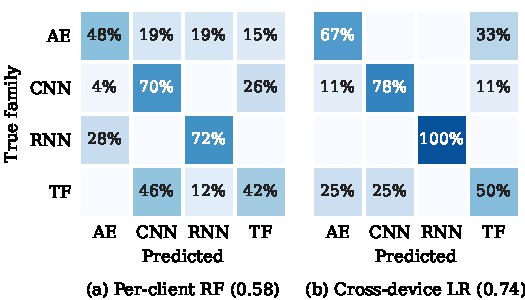
\includegraphics[width=\columnwidth]{fig_family_before_after.pdf}
\caption{Family confusion matrices for (a) the per-client baseline and (b) the
cross-device representation (leave-one-model-out). Cells give the percentage of
each true family assigned to each predicted family; empty cells are zero.
Balanced accuracy in parentheses.}
\label{fig:family_confusion}
\end{figure}

\subsection{Architecture Identification}
Using packet-morphology features, the architecture is identified within each
family well above chance (Table~\ref{tab:architecture_methods}). Recurrent architectures are separated
perfectly (1.00), autoencoder architectures reach 0.89, and convolutional
architectures 0.78. Transformer architectures are the most difficult (0.47),
partly because DistilBERT is represented by a single model. The mean across
families is 0.79 (macro F1 0.78), and the cross-device representation raises
convolutional architectures further to 0.81.

\begin{table}[!htbp]
\centering
\caption{Architecture Identification Within Each Family (Balanced Accuracy)}
\label{tab:architecture_methods}
\scriptsize
\renewcommand{\arraystretch}{1.08}
\setlength{\tabcolsep}{3pt}
\begin{tabular}{lccccc}
\hline
\textbf{Method} & \textbf{AE} & \textbf{CNN} & \textbf{RNN} & \textbf{Transf.} & \textbf{Mean} \\
\hline
Per-client RF (packet) & \textbf{0.89} & 0.78 & \textbf{1.00} & \textbf{0.47} & \textbf{0.79} \\
Cross-device LR & 0.67 & \textbf{0.81} & \textbf{1.00} & 0.25 & 0.68 \\
\hline
Chance          & 0.33 & 0.33 & 0.50 & 0.33 & -- \\
\hline
\end{tabular}
\end{table}

\subsection{Variant Identification}
At the finest level of the hierarchy, the uploaded payload size provides a
baseline leak. It is recovered from traffic within a median relative error of
$0.025\%$ of the true serialized size. Because every variant has a distinct
size, nearest-reference matching identifies the exact variant in all 90 traces
(chance $3.4\%$). Table~\ref{tab:variant_results} summarizes
the result per family.
Accounting for the client-specific header length is essential: assuming a single
header length under-counts the Windows client's payload by $0.8\%$ and causes
three of the 90 identifications to fail. Within a 5~s window, every variant with a short download is
identified, including all recurrent networks, autoencoders, MobileNets, and Tiny
Transformers, whereas EfficientNet, ResNet, and larger BERT downloads exceed the
window.

\begin{table}[!htbp]
\centering
\caption{Variant Identification by Payload Size}
\label{tab:variant_results}
\scriptsize
\renewcommand{\arraystretch}{1.05}
\setlength{\tabcolsep}{3pt}
\begin{tabular}{lcccc}
\hline
\textbf{Family} & \textbf{Traces} & \textbf{Payload (MB)} & \textbf{Trace} & \textbf{5~s} \\
\hline
Autoencoder & 27 & 0.01--10.1  & 1.00 & 0.96 \\
CNN         & 24 & 6.2--170.7  & 1.00 & 0.25 \\
RNN         & 18 & 0.22--2.2   & 1.00 & 1.00 \\
Transformer & 21 & 6.8--373.8  & 1.00 & 0.57 \\
\hline
\textbf{Total} & \textbf{90} & & \textbf{1.00} & \textbf{0.69} \\
\hline
\end{tabular}

\vspace{2pt}
\parbox{0.95\columnwidth}{\scriptsize Nearest-reference matching on log payload
size; 5~s: one complete download within a 5~s window. ResNet-34 and DistilBERT
are excluded (incomplete capture).}
\end{table}

\subsection{Discriminative Features}
\label{subsec:features}
Fisher scores computed on all observations indicate which features drive each
task; during evaluation, features are selected within each training fold. Transmission rates separate
families in per-client traces, whereas the cross-device representation relies on
burst and packet-size dispersion, led by the laptop's view of the same model.
The compute-timing features rank first for architecture identification in three
of the four families, through the compute gap per megabyte for autoencoders and
the cross-device gap ratio for recurrent networks and transformers.


\subsection{Short Observation Windows}
Table~\ref{tab:window_results} reports all three levels for single windows of
0.5 to 5~s and for longer observation times of 10 to 30~s. For family identification, single-client windows reach only 0.26--0.31 per
window, whereas concatenating the three clients' time-aligned windows, removing
near-idle windows, and classifying with logistic regression reaches 0.41 per
window at 0.5~s, rising to 0.51 at 5~s, and 0.51--0.65 after averaging window
posteriors per experiment. The cross-device gain is consistent across all window
sizes. The same representation identifies convolutional architectures with
0.65--0.71 per window and 0.89 after pooling at every window size, and
autoencoder architectures with up to 0.78 after pooling; recurrent and
transformer architectures, each represented by few models, are not reliably
identifiable from short windows. Variant identification requires a complete
model transfer within the window. Because model downloads are faster than
uploads on the testbed, a window that begins at a download identifies the exact
variant in $23\%$ of traces at 0.5~s, rising to $69\%$ at 5~s, and identifies
it correctly whenever the download completes within the window.

\begin{table}[!htbp]
\centering
\caption{Accuracy Versus Observation Time}
\label{tab:window_results}
\scriptsize
\renewcommand{\arraystretch}{1.08}
\setlength{\tabcolsep}{2pt}
\begin{tabular}{lcccc|cccc}
\hline
& \multicolumn{4}{c|}{\textbf{Single window}} & \multicolumn{4}{c}{\textbf{Accumulated}} \\
\textbf{Task} & \textbf{0.5~s} & \textbf{1~s} & \textbf{2~s} & \textbf{5~s} & \textbf{10~s} & \textbf{15~s} & \textbf{20~s} & \textbf{30~s} \\
\hline
Family, single client     & 0.26 & 0.29 & 0.30 & 0.31 & 0.31 & 0.31 & 0.30 & 0.30 \\
\textbf{Family, cross-device} & \textbf{0.41} & \textbf{0.43} & \textbf{0.46} & \textbf{0.51} & \textbf{0.53} & \textbf{0.54} & \textbf{0.55} & \textbf{0.56} \\
\hline
Arch., autoencoder         & 0.50 & 0.52 & 0.45 & 0.47 & 0.48 & 0.48 & 0.48 & 0.47 \\
Arch., CNN                 & 0.65 & 0.67 & 0.69 & 0.71 & 0.76 & 0.78 & 0.80 & 0.81 \\
Arch., RNN                 & 0.54 & 0.51 & 0.39 & 0.35 & 0.29 & 0.29 & 0.27 & 0.28 \\
Arch., transformer         & 0.21 & 0.22 & 0.20 & 0.19 & 0.20 & 0.19 & 0.19 & 0.19 \\
\hline
Variant$^{\dagger}$        & 0.23 & 0.32 & 0.39 & 0.69 & 0.80 & 0.82 & 0.86 & 0.90 \\
\hline
\end{tabular}

\vspace{2pt}
\parbox{0.95\columnwidth}{\scriptsize Balanced accuracy per decision. Family and
architecture: cross-device LR with near-idle windows removed, experiment-disjoint
5-fold CV grouped by model; 10--30~s average the posteriors of consecutive 5~s
windows over non-overlapping spans. Chance 0.25 (family), 0.33 (autoencoder,
CNN, transformer), 0.50 (RNN). $^{\dagger}$Share of traces whose variant is
identified from one complete download within the observation time.}
\end{table}

Accumulating evidence over longer observation helps where the per-window signal
is consistent (Table~\ref{tab:window_results}). Averaging the posteriors of
consecutive 5~s windows raises cross-device family accuracy from 0.51 at 5~s to
0.56 at 30~s and convolutional architecture accuracy from 0.71 to 0.81, whereas
the single-client baseline remains at 0.30--0.31 and autoencoder architecture
does not improve. Variant identification, which depends on capturing a complete
download, rises from $69\%$ of traces at 5~s to $90\%$ at 30~s.


\subsection{Ablation}
\label{subsec:ablation}
Table~\ref{tab:ablation} isolates the components of the proposed model under the
same leave-one-model-out protocol with nested selection. Neither component helps
in isolation: the cross-device representation with a random forest reaches 0.45,
and a per-client logistic regression also reaches 0.45, both below the per-client
random forest (0.58). Combined, they reach 0.74. Concatenating the three devices
yields few high-dimensional examples, which tree ensembles overfit but a
regularized linear model exploits. The compute-timing features contribute a
further 0.15 (0.59 without them). For short windows, the cross-device
representation improves both classifiers (5~s per-window accuracy from 0.31 to
0.44 with a random forest and from 0.35 to 0.49 with logistic regression), and
removing near-idle windows adds 0.02 per window. The cross-device gain does not
depend on a single device: with the laptop removed, combining the remaining two
devices still reaches 0.71 (95\% CI 0.57--0.85). As an upper bound, excluding
the ten variants whose compute profiles overlap another family (for example,
large ResNet and BERT models) and re-evaluating the round-level features on the
remaining 19 models raises nested leave-one-model-out family accuracy to 0.85;
because these exclusions were chosen from the observed errors, this figure bounds
the achievable accuracy rather than estimating generalization.

\begin{table}[!htbp]
\centering
\caption{Ablation of the Family Model (Balanced Accuracy)}
\label{tab:ablation}
\scriptsize
\renewcommand{\arraystretch}{1.08}
\setlength{\tabcolsep}{3pt}
\begin{tabular}{llccc}
\hline
\textbf{Representation} & \textbf{Classifier} & \textbf{Comp.} & \textbf{Bal. acc.} & \textbf{95\% CI} \\
\hline
\multicolumn{5}{l}{\textit{Complete trace (leave-one-model-out)}} \\
Per-client   & RF & \checkmark & 0.58 & 0.42--0.74 \\
Per-client   & LR & \checkmark & 0.45 & 0.34--0.56 \\
Cross-device & RF & \checkmark & 0.45 & 0.27--0.64 \\
Cross-device & LR & --         & 0.59 & 0.45--0.75 \\
\textbf{Cross-device} & \textbf{LR} & \checkmark & \textbf{0.74} & 0.58--0.88 \\
\hline
\multicolumn{5}{l}{\textit{5~s windows, per window / pooled}} \\
Single-client & RF & -- & \multicolumn{2}{c}{0.31 / 0.31} \\
Single-client & LR & -- & \multicolumn{2}{c}{0.35 / 0.40} \\
Cross-device  & RF & -- & \multicolumn{2}{c}{0.44 / 0.45} \\
Cross-device  & LR & -- & \multicolumn{2}{c}{0.49 / 0.62} \\
\textbf{Cross-device}$^{\dagger}$ & \textbf{LR} & -- & \multicolumn{2}{c}{\textbf{0.51 / 0.62}} \\
\hline
\end{tabular}

\vspace{2pt}
\parbox{0.95\columnwidth}{\scriptsize Comp.: compute-timing features.
$^{\dagger}$Near-idle windows removed. Windows: experiment-disjoint 5-fold CV
grouped by model.}
\end{table}

\subsection{Robustness to Size Padding}
\label{subsec:padding}
Padding every transfer to a size bucket defeats variant identification:
accuracy falls from 1.00 to 0.60 with 1~MB buckets ($1.8\%$ byte overhead),
to 0.45 with power-of-two buckets ($47\%$), and to chance (0.03) when all
transfers are padded to the largest model, at $1{,}086\%$ overhead. Family identification is unaffected, because the
compute gap and cross-device timing ratios do not depend on transfer size: using
these timing features alone, cross-device family identification reaches 0.62
(95\% CI 0.45--0.78, $p = 0.005$), matching the same model with size features
(0.60). Concealing model identity therefore requires timing defenses in addition
to size padding.


\subsection{Summary}
The cross-device timing signature reveals the family of unseen models (0.74),
also from short windows (0.51 per 5~s window, where it also identifies
convolutional architectures with 0.71), and remains effective under padding
(0.62). Within a family, packet-morphology features identify the architecture
with a mean balanced accuracy of 0.79. Payload size reveals the exact variant
(1.00, and 0.69 from a single download within a 5~s window), although padding
removes this signal.

\section{Countermeasures}
\label{sec:discussion}
Size padding removes the size-based variant signal (Sec.~\ref{subsec:padding}) but at a
substantial cost: padding every transfer to the largest model increases traffic
by $1{,}086\%$, whereas inexpensive 1~MB buckets still allow $60\%$
identification. Family leakage stems from timing, so effective defenses must
decouple traffic timing from local computation. Candidate defenses include
(i)~deadline-based rounds, in which every client uploads at a fixed time after
the download regardless of when training ends, hiding the compute gap at the
cost of round latency; (ii)~randomized upload delays, which blur the gap but
must be large relative to its variation across families; (iii)~cover traffic or
traffic shaping that keeps the link active during local training; and
(iv)~relaying updates through an intermediary that batches uploads from several
clients. Transport encryption and secure aggregation~\cite{TODO-secure-aggregation}
protect update contents but leave transfer timing unchanged. Quantifying the
privacy and latency trade-offs of these timing defenses is left for future work.


% Stub so the Introduction's reference resolves in this compile check.
\section{Conclusion}
\label{sec:conclusion}
Conclusion goes here.

\end{document}
